\chapter{Resultados y análisis}
\label{capitulo6}
\lhead{Capítulo 6. \emph{Resultados y análisis}}

\section{Pruebas en el EuRoC MAV Dataset}
A continuación se presentan los resultados obtenidos
utilizando las secuencias de datos  $MH\_ 01\_ easy$,  $MH\_ 05\_ difficult$,  $V1\_ 01\_ easy$,
$V1\_ 02\_ medium$ y  $V1\_ 03\_ difficult$, pertenecientes al EuRoC MAV Dataset.

En primera instancia se presentan los resultados directos del método iterativo de Gauss-Newton, y posteriormente los resultados obtenidos con la inicialización de este método utilizando los residuales de rotación provenientes del filtro inercial. Posteriormente se presentan los resultados obtenidos mediante el método RANSAC para la estimación del vector unitario de traslación.


\subsection{Evaluación del método de optimización de Gauss-Newton }

Para evaluar la estimación del método de Gauss-Newton se utilizó la secuencia $V1\_ 01\_ easy$ debido a que es una secuencia que presenta movimientos lentos y con mayor solapamiento entre imágenes, lo cual era un requisito para el método utilizado, ya que este utiliza un método directo para estimar la rotación y la traslación del robot. Los resultados de la orientación estimada de la cámara se presentan en la figura \ref{imagen:Resultados/GaussNewton/Orientacion}. En esta prueba se utilizó el detector SIFT y se utilizaron 4 escalas piramidales con un máximo número de iteraciones fijado a 10 para cada nivel. El tiempo promedio de estimación entre cada par de imágenes fue de 0.573243 s.

\begin{figure}[H]
	\centering
	\includegraphics[scale=0.6]{Resultados/GaussNewton/Orientacion}
	\caption[Orientación estimada con el]{Orientación estimada de la cámara con el método de optimización de Gauss-Newton en secuencia $V1\_ 01\_ easy$. }
	\label{imagen:Resultados/GaussNewton/Orientacion}
\end{figure}

 La figura \ref{imagen:Resultados/GaussNewton/Posicion} muestra los resultados de la posición estimada, la cual se encuentra escalada con el desplazamiento real obtenido del groundtruth. 
 

\begin{figure}[H]
	\centering
	\includegraphics[scale=0.6]{Resultados/GaussNewton/Posicion}
	\caption{Posición estimada de la cámara con el método de optimización de Gauss-Newton en secuencia $V1\_ 01\_ easy$. }
	\label{imagen:Resultados/GaussNewton/Posicion}
\end{figure}

Con estos resultados es posible concluir que el método empleado diverge, ya que la orientación estimada no posee cambios, lo cual también se evidencia en la estimación de la posición de la cámara  en la figura \ref{imagen:Resultados/GaussNewton/Posicion}.

\subsubsection{Inicialización con residuales inerciales}
Debido a la divergencia del método de Gauss-Newton, se evaluaron nuevamente los resultados del método utilizando los residuales inerciales,  bajo la premisa de obtener estimaciones convergentes al inicializar el método en una estimación del movimiento rotacional más cercana a la real.

Los residuales inerciales y la orientación del robot provienen del filtro inercial. En la figura \ref{imagen:Resultados/GaussNewtonConResiduales1/ResidualOrientacionHistograma} se presentan los residuales inerciales utilizados en la inicialización. La figura \ref{imagen:Resultados/GaussNewtonConResiduales1/ErrorResidualOrientacion} muestra el error del residual y el error de orientación  se presenta en la figura \ref{imagen:Resultados/GaussNewtonConResiduales1/ErrorOrientacion}.

\begin{figure}[H]
	\centering
	\includegraphics[scale=0.6]{Resultados/GaussNewtonConResiduales1/ResidualOrientacionHistograma}
	\caption{ Residual de orientación estimado en secuencia $V1\_ 01\_ easy$.}
	\label{imagen:Resultados/GaussNewtonConResiduales1/ResidualOrientacionHistograma}
\end{figure}

\begin{figure}[H]
	\centering
	\includegraphics[scale=0.6]{Resultados/GaussNewtonConResiduales1/ErrorResidualOrientacion}
	\caption{ Error del residual de orientación estimado en secuencia $V1\_ 01\_ easy$.}
	\label{imagen:Resultados/GaussNewtonConResiduales1/ErrorResidualOrientacion}
\end{figure}

\begin{figure}[H]
	\centering
	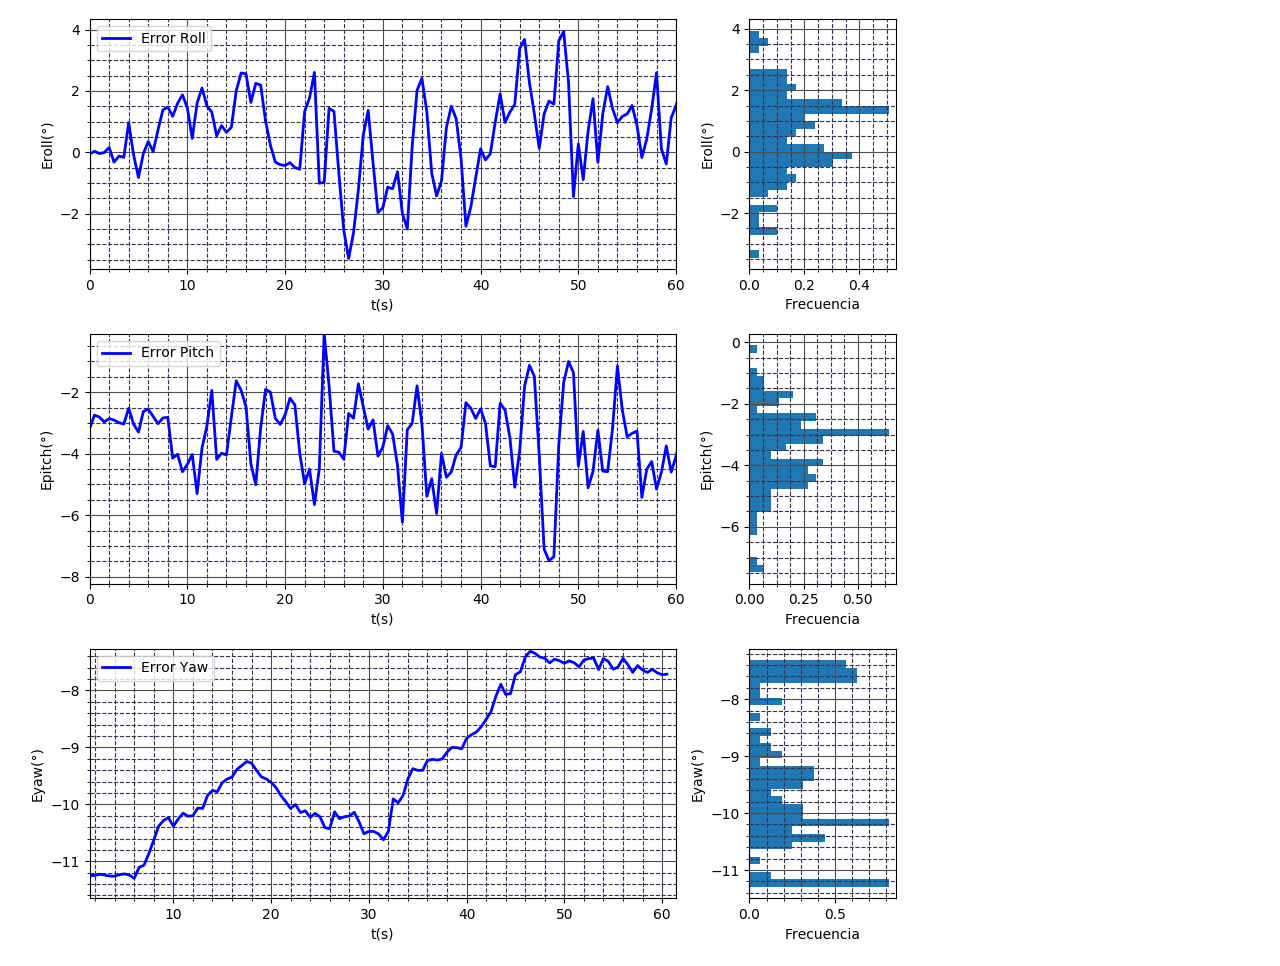
\includegraphics[scale=0.6]{Resultados/GaussNewtonConResiduales1/ErrorOrientacion}
	\caption{Posición estimada de la cámara con el método de optimización de Gauss-Newton en secuencia $V1\_ 01\_ easy$ empleando residuales inerciales. }
	\label{imagen:Resultados/GaussNewtonConResiduales1/ErrorOrientacion}
\end{figure}

Finalmente los resultados de la estimación de la posición se presentan en la figura \ref{imagen:Resultados/GaussNewtonConResiduales1/Posicion}.

\begin{figure}[H]
	\centering
	\includegraphics[scale=0.6]{Resultados/GaussNewtonConResiduales1/Posicion}
	\caption{Posición estimada de la cámara con el método de optimización de Gauss-Newton en secuencia $V1\_ 01\_ easy$ empleando residuales inerciales. }
	\label{imagen:Resultados/GaussNewtonConResiduales1/Posicion}
\end{figure}

En este caso la prueba realizada fue similar y se obtuvo un tiempo promedio de iteración del algoritmo de 0.799779 s, el cual es mayor al presentado sin la inicialización con residuales. En primer lugar esto indica que el algoritmo itera un mayor número de veces de la solución que minimice el error fotométrico. Es posible observar que la orientación de la cámara en este caso si es seguida debido a que el error de orientación se mantiene pequeño en los ángulos de roll y pitch, y sufre de drift en el angulo de yaw, lo cual se debe a que esta orientación es principalmente la orientación que se obtiene del filtro inercial. Sin embargo los resultados de la estimación de la posición no fueron satisfactorios.

También es posible observar en los histogramas de las figuras \ref{imagen:Resultados/GaussNewtonConResiduales1/ResidualOrientacionHistograma} y \ref{imagen:Resultados/GaussNewtonConResiduales1/ErrorResidualOrientacion} que el error porcentual del residual es relativamente alto para movimientos lentos, ya que en esta prueba la estimación de residuales se realiza imagen por imagen. Por estas razones, se realizó una segunda prueba calculando los residuales e inicializando el algoritmo de estimación cada 10 imágenes para comparar la estimación de la posición y el error de los residuales. En las figuras  \ref{imagen:Resultados/GaussNewtonConResiduales10/ResidualOrientacionHistograma}, \ref{imagen:Resultados/GaussNewtonConResiduales10/ErrorResidualOrientacion} y \ref{imagen:Resultados/GaussNewtonConResiduales10/Posicion} se muestran los resultados.

\begin{figure}[H]
	\centering
	\includegraphics[scale=0.6]{Resultados/GaussNewtonConResiduales10/ResidualOrientacionHistograma}
	\caption{ Residual de orientación estimado en secuencia $V1\_ 01\_ easy$.}
	\label{imagen:Resultados/GaussNewtonConResiduales10/ResidualOrientacionHistograma}
\end{figure}

\begin{figure}[H]
	\centering
	\includegraphics[scale=0.6]{Resultados/GaussNewtonConResiduales10/ErrorResidualOrientacion}
	\caption{ Error del residual de orientación estimado en secuencia $V1\_ 01\_ easy$.}
	\label{imagen:Resultados/GaussNewtonConResiduales10/ErrorResidualOrientacion}
\end{figure}


\begin{figure}[H]
	\centering
	\includegraphics[scale=0.6]{Resultados/GaussNewtonConResiduales10/Posicion}
	\caption{Posición estimada de la cámara con el método de optimización de Gauss-Newton en secuencia $V1\_ 01\_ easy$ empleando residuales inerciales. }
	\label{imagen:Resultados/GaussNewtonConResiduales10/Posicion}
\end{figure}

En esta prueba se tuvo un tiempo promedio de 0.739407 s y se puedo observar que el error porcentual de los residuales es más pequeño. Esto indicó que los residuales de orientación tendían a ser más exactos a mayores rangos de movimiento rotacional, lo cual los hace incompatibles con el método de optimización empleado ya que este requiere rangos mínimos de movimiento, lo cual se comprueba nuevamente con la divergencia de la estimación de la posición.

\subsection{Evaluación del método RANSAC}

En la evaluación del metodo de dos puntos se utilizaron secuencias lentas $MH\_ 01\_ easy$ y $V1\_ 01\_ easy$ y la secuencia rápida $V1\_ 02\_ medium$, para comparar el desempeño de los diferentes detectores ante cambios bruscos de movimiento. 

En este caso se utilizaron los detectores KAZE, AKAZE, ORB, SIFT y SURF en la evaluación. Las siguente secciones presentan los resultados de rendimiento de cada detector.

 Además se presentan las gráficas de posición, error de orientación y residuales de velocidad del detector con mejor estimación del conjunto y del detector con mejor eficiencia computacional. Esto, a manera de resumen debido a que la orientación y los residuales de velocidad en general son similares en cada detector empleado, ya que dependen en mayor medida del filtro inercial.  El conjunto total de gráficas de resultados para cada detector pueden ser visualizadas en la sección de resultados del  \href{https://github.com/Lujano/tesis/tree/master/imagenes/Resultados/}{\underline{repositorio del libro de tesis}}.
 
 
En cada sección se presentan los parámetros de configuración utilizados para la ejecución del sistema, como el umbral del RANSAC, el número de frames estáticos, el umbral para las disparidades euclidiana, rotacional y traslacional, y el umbral definido al detector utilizado. 
 
 El umbral del RANSAC representa el valor absoluto del máximo valor permisible del resultado del producto punto del vector de traslación estimado y el vector normal al plano epipolar de un punto característico, para ser clasificado como inlier. Es decir, si el valor absuluto del resultado es menor al umbral, el vector normal generado por la pareja de puntos característicos es clasificado dentro del modelo (inlier).
 
 La disparidad euclidiana es el promedio de distancia en unidades de píxeles de las parejas de puntos característicos en cada imagen. Un frame es considerado estático cuando no es keyframe y la disparidad euclidiana se encuentra por debajo del valor del umbral.
 
 El número de frames estáticos representa el número mínimo de imágenes seguidas que deben ser clasificadas como frame estático para que el movimiento del robot sea clasificado como estático. Cuando esto ultimo ocurre, el bias de la imu es calculado.

 Por su parte, una imagen es considerada como keyframe cuando la disparidad rotacional o traslacional excede su umbral.
 
 En el caso del umbral del detector es el valor de umbral de cada detector en las funciones de Opencv, el cual afecta el número de features detectados. En este caso, este valor umbral es seleccionado de forma tal que el número de features promedio detectados en la secuencia sea similar en todos los detectores. De esta forma, el análisis de datos de los resultados se puede realizar bajo condiciones similares.

\subsubsection{Secuencia Machine Hall Easy}


La tabla \ref{Tabla/Parametros/MH_01_easy} presenta los parámetros de configuración inicial del sistema empleados en esta secuencia. Los umbrales seleccionados fueron seleccionados de forma empírica. En particular, el umbral de los detectores es eligido para generar un aproximado de 100 puntos característicos por imagen.

\begin{table}[H]
	\caption{Parámetros de configuración en Secuencia $MH\_ 01\_ easy$.}
	\begin{tabular}{|l|c|c|c|c|c|}
		\hline
		\multicolumn{1}{|c|}{\textbf{Detector}} & \textbf{KAZE} & \textbf{AKAZE} & \textbf{ORB} & \textbf{SIFT} & \textbf{SURF} \\ \hline
		Umbral del RANSAC & 0.18 & 0.18 & 0.18 & 0.18 & 0.18 \\ \hline
		Umbral de frames estáticos & 4 & 4 & 4 & 4 & 4 \\ \hline
		Umbral disparidad euclideana & 0.5 & 0.5 & 0.5 & 0.5 & 0.5 \\ \hline
		Umbral disparidad rotacional (°) & 5 & 5 & 5 & 5 & 5 \\ \hline
		Umbral disparidad traslacional (px) & 15 & 15 & 15 & 15 & 15 \\ \hline
		Umbral del detector & 0.012 & 0.012 & 100 & 100 & 10000 \\ \hline
	\end{tabular}
	\label{Tabla/Parametros/MH_01_easy}
\end{table}


La tabla \ref{Tabla/Resultados/MH_01_easy} presenta los resultados obtenidos para la secuencia Machine Hall Easy. En particular  se puede observar que el número de parejas iniciales  promedio antes de aplicar el filtro de celdas es mayor para los detectores KAZE y SURF. Por el contrario, ORB presenta el menor porcentaje de parejas iniciales generadas respecto al número de puntos característicos. Esto implica que los detectores KAZE y SURF presentan mejor relación de parejas generadas por puntos característicos detectados en esta secuencia. Esto también es reflejado en las estadísticas del número de \textit{inliers} del RANSAC.  Sin embargo, el detector ORB es el más rápido de los detectores al tener 30.5 ms de tiempo promedio de detección.

Es posible observar que el tiempo de estimación del vector de traslación unitario es de aproximadamente 0.3 ms, lo cual comparado con los 0.73 s del método de optimización de Gauss-Newton, es cerca de 2400 veces más rápido. Se puede observar además que el sistema implementado corre en tiempo real en el caso de utilizar el detector ORB, donde el tiempo de procesamiento para todo la secuencia de 105 s de duración es de 79.8 s.


\begin{table}[H]
	\caption{Resultados en Secuencia $MH\_ 01\_ easy$.}
	\begin{tabular}{|l|c|c|c|c|c|}
		\hline
		\multicolumn{1}{|c|}{\textbf{Detector}} & \textbf{KAZE} & \textbf{AKAZE} & \textbf{ORB} & \textbf{SIFT} & \textbf{SURF} \\ \hline
		Número de features detectados & 113 & 111 & 100 & 100 & 119 \\ \hline
		Número de parejas iniciales & 73 & 61 & 37 & 62 & 80 \\ \hline
		Número de parejas del filtro de celdas & 28 & 21 & 12 & 29 & 31 \\ \hline
		Número de inliers del RANSAC & 53 & 43 & 24 & 45 & 58 \\ \hline
		Número de imágenes procesadas & 2099 & 2099 & 2099 & 2099 & 2099 \\ \hline
		Número de keyframes & 342 & 297 & 396 & 518 & 497 \\ \hline
		Tiempo promedio de filtro inercial (ms) & 5.5 & 6.1 & 6.1 & 5.7 & 6.0 \\ \hline
		Tiempo promedio de detección  (ms) & 743.2 & 166.9 & 30.5 & 346.9 & 116.7 \\ \hline
		Tiempo promedio de match (ms) & 1.9 & 2.6 & 1.3 & 1.7 & 2.1 \\ \hline
		Tiempo promedio de RANSAC (ms) & 0.3 & 0.3 & 0.2 & 0.3 & 0.3 \\ \hline
		Tiempo de estimación (s) & 11.7 & 12.8 & 13.0 & 12.2 & 12.8 \\ \hline
		Tiempo de  procesamiento (s) & 1574.4 & 367.1 & 79.8 & 743.5 & 262.3 \\ \hline
		Tiempo de evaluación (s) & 105.0 & 105.0 & 105.0 & 105.0 & 105.0 \\ \hline
	\end{tabular}
	\label{Tabla/Resultados/MH_01_easy}
\end{table}



\paragraph {KAZE \\ \\}


En la figuras \ref{imagen:Resultados/MH_01_easy/KAZE/Posicion} y \ref{imagen:Resultados/MH_01_easy/KAZE/Orientacion} y \ref{imagen:Resultados/MH_01_easy/KAZE/ResidualVelocidad} se presentan los resultados de posición estimada del vehículo áreo. En este caso la escala de desplazamiento es tomada del \textit{groundtruth} debido al fallo de las triangulaciones realizadas por el sistema.
 
\begin{figure}[H]
	\centering
	\includegraphics[scale=0.6]{Resultados/MH_01_easy/KAZE/Posicion}
	\caption{Posición de la cámara KAZE}
	\label{imagen:Resultados/MH_01_easy/KAZE/Posicion}
\end{figure}

Es posible observar que la estimación de la posición escalada se realiza de forma efectiva  en $x$ y $y$, mientras que en $z$ se observa un mayor efecto de la acumulación de errores de estimación entre \textit{keyframes} (\textit{drift}).


\begin{figure}[H]
	\centering
	\includegraphics[scale=0.6]{Resultados/MH_01_easy/KAZE/Orientacion}
	\caption[Error de Orientación KAZE]{Error de Orientación KAZE.}
	\label{imagen:Resultados/MH_01_easy/KAZE/Orientacion}
\end{figure}

Por su parte el error de orientación de la orientación estimada se mantiene acotado, y es importante observar que el \textit{drift} en el ángulo de \textit{yaw} es pequeño a pesar de los 120 s de duración aproximada de la secuencia. Además los histogramas del error en \textit{pitch} y \textit{roll} presentan una media de cero. Esto expone el buen funcionamiento del módulo de seguimiento de \textit{bias} en esta secuencia. 

\begin{figure}[H]
	\centering
	\includegraphics[scale=0.6]{Resultados/MH_01_easy/KAZE/ResidualVelocidad2}
	\caption{Residual de velocidad KAZE}
	\label{imagen:Resultados/MH_01_easy/KAZE/ResidualVelocidad}
\end{figure}

%
%\subsubsection{AKAZE}
%
%
%\begin{figure}[H]
%	\centering
%	\includegraphics[scale=0.6]{Resultados/MH_01_easy/AKAZE/Posicion}
%	\caption{Posición de la cámara AKAZE}
%	\label{imagen:Resultados/MH_01_easy/AKAZE/Posicion}
%\end{figure}
%
%
%\begin{figure}[H]
%	\centering
%	\includegraphics[scale=0.6]{Resultados/MH_01_easy/AKAZE/Orientacion}
%	\caption[Error de Orientación AKAZE]{Error de Orientación AKAZE.}
%	\label{imagen:Resultados/MH_01_easy/AKAZE/Orientacion}
%\end{figure}
%
%
%
%\begin{figure}[H]
%	\centering
%	\includegraphics[scale=0.6]{Resultados/MH_01_easy/AKAZE/ResidualVelocidad2}
%	\caption{Residual de velocidad AKAZE}
%	\label{imagen:Resultados/MH_01_easy/AKAZE/ResidualVelocidad}
%\end{figure}

\paragraph {ORB \\ \\}

En el caso del detector ORB , los resultados son similares a los obtenidos con el detector KAZE. En la figura \ref{imagen:Resultados/MH_01_easy/ORB/Posicion} se presenta los resultados de la posición estimada.
	
\begin{figure}[H]
	\centering
	\includegraphics[scale=0.6]{Resultados/MH_01_easy/ORB/Posicion}
	\caption{Posición de la cámara ORB}
	\label{imagen:Resultados/MH_01_easy/ORB/Posicion}
\end{figure}

De esta forma es posible concluir que el método RANSAC con el detector ORB presentó la mejor relación entre precisión de la estimación y tiempo de procesamiento, logrando la estimación del movimiento del vehículo en tiempo real.

%\begin{figure}[H]
%	\centering
%	\includegraphics[scale=0.6]{Resultados/MH_01_easy/ORB/Orientacion}
%	\caption[Error de Orientación ORB]{Error de Orientación ORB.}
%	\label{imagen:Resultados/MH_01_easy/ORB/Orientacion}
%\end{figure}
%\begin{figure}[H]
%	\centering
%	\includegraphics[scale=0.6]{Resultados/MH_01_easy/ORB/ResidualVelocidad2}
%	\caption{Residual de velocidad ORB}
%	\label{imagen:Resultados/MH_01_easy/ORB/ResidualVelocidad}
%\end{figure}


%\subsubsection{SIFT}
%
%
%\begin{figure}[H]
%	\centering
%	\includegraphics[scale=0.6]{Resultados/MH_01_easy/SIFT/Posicion}
%	\caption{Posición de la cámara SIFT}
%	\label{imagen:Resultados/MH_01_easy/SIFT/Posicion}
%\end{figure}
%
%
%\begin{figure}[H]
%	\centering
%	\includegraphics[scale=0.6]{Resultados/MH_01_easy/SIFT/Orientacion}
%	\caption[Error de Orientación SIFT]{Error de Orientación SIFT.}
%	\label{imagen:Resultados/MH_01_easy/SIFT/Orientacion}
%\end{figure}
%
%
%
%\begin{figure}[H]
%	\centering
%	\includegraphics[scale=0.6]{Resultados/MH_01_easy/SIFT/ResidualVelocidad2}
%	\caption{Residual de velocidad SIFT}
%	\label{imagen:Resultados/MH_01_easy/SIFT/ResidualVelocidad}
%\end{figure}
%
%\subsubsection{SURF}
%
%
%\begin{figure}[H]
%	\centering
%	\includegraphics[scale=0.6]{Resultados/MH_01_easy/SURF/Posicion}
%	\caption{Posición de la cámara SURF}
%	\label{imagen:Resultados/MH_01_easy/SURF/Posicion}
%\end{figure}
%
%
%\begin{figure}[H]
%	\centering
%	\includegraphics[scale=0.6]{Resultados/MH_01_easy/SURF/Orientacion}
%	\caption[Error de Orientación SURF]{Error de Orientación SURF.}
%	\label{imagen:Resultados/MH_01_easy/SURF/Orientacion}
%\end{figure}
%
%
%
%\begin{figure}[H]
%	\centering
%	\includegraphics[scale=0.6]{Resultados/MH_01_easy/SURF/ResidualVelocidad2}
%	\caption{Residual de velocidad SURF}
%	\label{imagen:Resultados/MH_01_easy/SURF/ResidualVelocidad}
%\end{figure}
%


\subsubsection{Vicon Room Easy}

La configuración inicial de los detectores se presenta en la tabla \ref{Tabla/Parametros/V1_01_easy}. En este caso los umbrales de los detectores KAZE, AKAZE y SURF fueron modificados para generar un mayor número de puntos característicos.

\begin{table}[H]
	\caption{Parámetros de configuración en secuencia $V1\_01\_easy$.}
	\begin{tabular}{|l|c|c|c|c|c|}
		\hline
		\multicolumn{1}{|c|}{\textbf{Detector}} & \textbf{KAZE} & \textbf{AKAZE} & \textbf{ORB} & \textbf{SIFT} & \textbf{SURF} \\ \hline
		Umbral del RANSAC & 0.18 & 0.18 & 0.18 & 0.18 & 0.18 \\ \hline
		Umbral de frames estáticos & 4 & 4 & 4 & 4 & 4 \\ \hline
		Umbral disparidad euclideana & 0.5 & 0.5 & 0.5 & 0.5 & 0.5 \\ \hline
		Umbral disparidad rotacional (°) & 5 & 5 & 5 & 5 & 5 \\ \hline
		Umbral disparidad traslacional (px) & 15 & 15 & 15 & 15 & 15 \\ \hline
		Umbral del detector & 0.008 & 0.006 & 100 & 100 & 6000 \\ \hline
	\end{tabular}
	\label{Tabla/Parametros/V1_01_easy}
\end{table}

La tabla \ref{Tabla/Resultados/V1_01_easy}  presenta los resultados estadísticos  obtenidos. Es posible ver que respecto a los resultados obtenidos en la secuencia Machine Hall Easy, al duplicar el número de puntos característicos del detector KAZE, el número de parejas promedio antes del filtrado son también duplicadas. Lo mismo ocurre en la misma proporción en los detectores AKAZE y SURF. 

Por otro lado es posible observar que el número de \textit{keyframes} generados en cada caso es mayor que en la secuencia anterior debido a que Vicon Room Easy presenta mayor movimiento ya que Machine Hall Easy presenta 40 s de movimiento estático inicial. 

\begin{table}[H]
	\caption{Resultados en secuencia $V1\_ 01\_ easy$.}
	\begin{tabular}{|l|c|c|c|c|c|}
		\hline
		\multicolumn{1}{|c|}{\textbf{Detector}} & \textbf{KAZE} & \textbf{AKAZE} & \textbf{ORB} & \textbf{SIFT} & \textbf{SURF} \\ \hline
		Número de features detectados & 230 & 243 & 100 & 100 & 150 \\ \hline
		Número de parejas iniciales & 153 & 136 & 35 & 61 & 103 \\ \hline
		Número de parejas del filtro de celdas & 26 & 23 & 9 & 13 & 26 \\ \hline
		Número de inliers del RANSAC & 93 & 76 & 19 & 32 & 67 \\ \hline
		Número de imágenes procesadas & 2498 & 2498 & 2498 & 2498 & 2498 \\ \hline
		Número de keyframes & 638 & 565 & 685 & 711 & 738 \\ \hline
		Tiempo promedio de filtro inercial (ms) & 5.9 & 6.2 & 6.8 & 6.2 & 6.6 \\ \hline
		Tiempo promedio de detección  (ms) & 764.6 & 181.6 & 27 & 337.7 & 128.7 \\ \hline
		Tiempo promedio de match (ms) & 6.4 & 11.9 & 1.4 & 1.8 & 3.2 \\ \hline
		Tiempo promedio de RANSAC (ms) & 0.6 & 0.5 & 0.2 & 0.3 & 0.4 \\ \hline
		Tiempo de estimación (s) & 15 & 15.9 & 17.1 & 15.6 & 16.8 \\ \hline
		Tiempo de  procesamiento (s) & 1936.3 & 497.5 & 88.1 & 862 & 262.3 \\ \hline
		Tiempo de evaluación (s) & 124.9 & 124.9 & 124.9 & 124.9 & 124.9 \\ \hline
	\end{tabular}
	\label{Tabla/Resultados/V1_01_easy}
\end{table}


En esta secuencia el detector con mejores resultados de estimación fue el detector KAZE. Respecto a desempeño computacional, el detector ORB presentó  el mejor desempeño. A continuación se presentan las gráficas de las estimaciones de movimiento de ambos detectores.
\paragraph {KAZE \\ \\}

Las figuras \ref{imagen:Resultados/V1_01_easy/KAZE/Posicion}  y \ref{imagen:Resultados/V1_01_easy/KAZE/Orientacion} presentan la posición y el error de orientación estimado utilizando el detector KAZE. En esta caso también se observa un seguimiento correcto de las posición estimada en los $x$ y $y$. En el caso de la altura estimada (eje $z$) podemos ver que existe un seguimiento inicial que es perdido en las estimaciones siguientes. Sin embargo el rango de movimiento en $z$ es mucho menor al presentado en $x$ y $y$.

\begin{figure}[H]
	\centering
	\includegraphics[scale=0.6]{Resultados/V1_01_easy/KAZE/Posicion}
	\caption{Posición de la cámara KAZE}
	\label{imagen:Resultados/V1_01_easy/KAZE/Posicion}
\end{figure}


Por su parte, la orientación estimada presenta buenos resultados. Esto se puede evidenciar en las gráficas del error de orientación estimado, donde el mayor error angular alcanza cerca de los 13 grados.

\begin{figure}[H]
	\centering
	\includegraphics[scale=0.6]{Resultados/V1_01_easy/KAZE/Orientacion}
	\caption[Error de Orientación KAZE]{Error de Orientación KAZE.}
	\label{imagen:Resultados/V1_01_easy/KAZE/Orientacion}
\end{figure}


En cuanto a los residuales de velocidad presentados en la figura \ref{imagen:Resultados/V1_01_easy/KAZE/ResidualVelocidad} se tiene que los mejores resultados se obtienen para el eje $z$, lo cual es un caso bastante común debido a que este residual depende unicamente del correcto seguimiento de los ángulos de \textit{roll} y \textit{pitch}, mientras que los residuales en $x$ y $y$ son más sensibles al ángulo de \textit{yaw} y de los sesgos del acelerómetro.


\begin{figure}[H]
	\centering
	\includegraphics[scale=0.6]{Resultados/V1_01_easy/KAZE/ResidualVelocidad2}
	\caption{Residual de velocidad KAZE}
	\label{imagen:Resultados/V1_01_easy/KAZE/ResidualVelocidad}
\end{figure}



%\subsubsection{AKAZE}
%
%
%\begin{figure}[H]
%	\centering
%	\includegraphics[scale=0.6]{Resultados/V1_01_easy/AKAZE/Posicion}
%	\caption{Posición de la cámara AKAZE}
%	\label{imagen:Resultados/V1_01_easy/AKAZE/Posicion}
%\end{figure}
%
%
%\begin{figure}[H]
%	\centering
%	\includegraphics[scale=0.6]{Resultados/V1_01_easy/AKAZE/Orientacion}
%	\caption[Error de Orientación AKAZE]{Error de Orientación AKAZE.}
%	\label{imagen:Resultados/V1_01_easy/AKAZE/Orientacion}
%\end{figure}
%
%
%
%\begin{figure}[H]
%	\centering
%	\includegraphics[scale=0.6]{Resultados/V1_01_easy/AKAZE/ResidualVelocidad2}
%	\caption{Residual de velocidad AKAZE}
%	\label{imagen:Resultados/V1_01_easy/AKAZE/ResidualVelocidad}
%\end{figure}

\paragraph {ORB \\ \\}

En esta secuencia los resultados de estimación de posición con el detector ORB presentan de forma más evidente el \textit{drift}, siendo más evidente en las estimaciones posteriores a los 80 segundos. Sin embargo, las estimación local de las traslaciones se mantiene producto de la correcta estimación de la orientación de la cámara. El detector ORB presenta de nuevo la mejor relación entre la calidad de las estimaciones traslacionales y tiempo computacional.

\begin{figure}[H]
	\centering
	\includegraphics[scale=0.6]{Resultados/V1_01_easy/ORB/Posicion}
	\caption{Posición de la cámara ORB}
	\label{imagen:Resultados/V1_01_easy/ORB/Posicion}
\end{figure}


%\begin{figure}[H]
%	\centering
%	\includegraphics[scale=0.6]{Resultados/V1_01_easy/ORB/Orientacion}
%	\caption[Error de Orientación ORB]{Error de Orientación ORB.}
%	\label{imagen:Resultados/V1_01_easy/ORB/Orientacion}
%\end{figure}
%\begin{figure}[H]
%	\centering
%	\includegraphics[scale=0.6]{Resultados/V1_01_easy/ORB/ResidualVelocidad2}
%	\caption{Residual de velocidad ORB}
%	\label{imagen:Resultados/V1_01_easy/ORB/ResidualVelocidad}
%\end{figure}

%
%\subsubsection{SIFT}
%
%
%\begin{figure}[H]
%	\centering
%	\includegraphics[scale=0.6]{Resultados/V1_01_easy/SIFT/Posicion}
%	\caption{Posición de la cámara SIFT}
%	\label{imagen:Resultados/V1_01_easy/SIFT/Posicion}
%\end{figure}
%
%
%\begin{figure}[H]
%	\centering
%	\includegraphics[scale=0.6]{Resultados/V1_01_easy/SIFT/Orientacion}
%	\caption[Error de Orientación SIFT]{Error de Orientación SIFT.}
%	\label{imagen:Resultados/V1_01_easy/SIFT/Orientacion}
%\end{figure}
%
%
%
%\begin{figure}[H]
%	\centering
%	\includegraphics[scale=0.6]{Resultados/V1_01_easy/SIFT/ResidualVelocidad2}
%	\caption{Residual de velocidad SIFT}
%	\label{imagen:Resultados/V1_01_easy/SIFT/ResidualVelocidad}
%\end{figure}

%\subsubsection{SURF}
%
%
%\begin{figure}[H]
%	\centering
%	\includegraphics[scale=0.6]{Resultados/V1_01_easy/SURF/Posicion}
%	\caption{Posición de la cámara SURF}
%	\label{imagen:Resultados/V1_01_easy/SURF/Posicion}
%\end{figure}
%
%
%\begin{figure}[H]
%	\centering
%	\includegraphics[scale=0.6]{Resultados/V1_01_easy/SURF/Orientacion}
%	\caption[Error de Orientación SURF]{Error de Orientación SURF.}
%	\label{imagen:Resultados/V1_01_easy/SURF/Orientacion}
%\end{figure}
%
%
%
%\begin{figure}[H]
%	\centering
%	\includegraphics[scale=0.6]{Resultados/V1_01_easy/SURF/ResidualVelocidad2}
%	\caption{Residual de velocidad SURF}
%	\label{imagen:Resultados/V1_01_easy/SURF/ResidualVelocidad}
%\end{figure}
%



\subsubsection{Vicon Room Medium}

La secuencia Vicon Room Medium presenta movimientos más dinámicos respecto a las secuencias Easy. Por tanto, se presentan con mayor frecuencia efectos de distorsión de la imagen como el \textit{blur}, que disminuyen el numero de puntos caracterísiticos que pueden ser detectados en una imagen. Debido a esto, los umbrales de detección presentados en la tabla \ref{Tabla/Parametros/V1_02_medium} son configurados para generar un mayor número de puntos característicos, tal como se muestra en la tabla \ref{Tabla/Resultados/V1_02_medium}.

Como consecuencia del aumento del número de número de puntos característicos promedio, se puede ver que el tiempo de emparejamiento (\textit{match}) a aumentado de 1.8 ms con 100 puntos característicos en la secuencia anterior en el caso de SIFT, a 6.6 ms con 247 puntos característicos en la secuencia actual, por lo que es evidente que el tiempo de emparejamiento no aumenta linealmente con el número de puntos de característicos a emparejar.

% Esto lleva a que en general se tomen estrategias para seleccionar la mejor cantidad de puntos característicos a detectar en función del tipo de modo de visión utilizado. Por ejemplo, en SLAM con visión estéreo son necesarios un número menor de puntos característicos por imagen que en visión monocular, ya que se puede triangular en cada imagen obtenida. Sin embargo, en visión monocular se necesitan más referencias de la escena ya que se debe seleccionar las imágenes más adecuadas para la triangulación.

\begin{table}[H]
	\caption{Parámetros de configuración  en secuencia $V1\_ 02\_ medium$.}
	\begin{tabular}{|l|c|c|c|c|c|}
		\hline
		\multicolumn{1}{|c|}{\textbf{Detector}} & \textbf{KAZE} & \textbf{AKAZE} & \textbf{ORB} & \textbf{SIFT} & \textbf{SURF} \\ \hline
		Umbral del RANSAC & 0.18 & 0.18 & 0.18 & 0.18 & 0.18 \\ \hline
		Umbral de frames estáticos & 4 & 4 & 4 & 4 & 4 \\ \hline
		Umbral disparidad euclideana & \textbf{1} & \textbf{1} & \textbf{1} & \textbf{1} & \textbf{1} \\ \hline
		Umbral disparidad rotacional (°) & 5 & 5 & 5 & 5 & 5 \\ \hline
		Umbral disparidad traslacional (px) & 15 & 15 & 15 & 15 & 15 \\ \hline
		Umbral del detector & 0.005 & 0.003 & 250 & 250 & 1100 \\ \hline
	\end{tabular}
	\label{Tabla/Parametros/V1_02_medium}
\end{table}

Una característica a resaltar de los resultados de la tabla \ref{Tabla/Resultados/V1_02_medium} es que la relación entre el número de \textit{keyframes} y el numero de imágenes de la secuencia (procesadas) es mayor en comparación con las secuencias lentas, lo cual es un resultado lógico debido a que al ser una secuencia de movimientos rápidos se tiene mayor disparidad entre imágenes sucesivas, lo que implica que los \textit{keyframes} son insertados de forma más frecuente en las estimaciones de movimiento.

Finalmente, se obtienen resultados similares sobre el desempeño del detector ORB, siendo el detector más eficiente computacionalmente.
 
\begin{table}[H]
	\caption{Resultados  en secuencia $V1\_02\_medium$.}
	\begin{tabular}{|l|c|c|c|c|c|}
		\hline
		\multicolumn{1}{|c|}{\textbf{Detector}} & \textbf{KAZE} & \textbf{AKAZE} & \textbf{ORB} & \textbf{SIFT} & \textbf{SURF} \\ \hline
		Número de features detectados & 227 & 261 & 249 & 247 & 353 \\ \hline
		Número de parejas iniciales & 142 & 146 & 81 & 150 & 230 \\ \hline
		Número de parejas del filtro de celdas & 30 & 27 & 15 & 35 & 45 \\ \hline
		Número de inliers del RANSAC & 96 & 89 & 48 & 100 & 163 \\ \hline
		Número de imágenes procesadas & 1625 & 1643 & 1644 & 1647 & 1647 \\ \hline
		Número de keyframes & 719 & 647 & 715 & 800 & 768 \\ \hline
		Tiempo promedio de filtro inercial (ms) & 5.4 & 6.5 & 6.8 & 6.1 & 6.3 \\ \hline
		Tiempo promedio de detección  (ms) & 699.4 & 192 & 25.8 & 348.5 & 202.6 \\ \hline
		Tiempo promedio de match (ms) & 4.2 & 10.4 & 4.6 & 6.6 & 9.8 \\ \hline
		Tiempo promedio de RANSAC (ms) & 0.5 & 0.6 & 0.4 & 0.6 & 1 \\ \hline
		Tiempo de estimación (s) & 9.2 & 11.1 & 11.4 & 10.5 & 11.1 \\ \hline
		Tiempo de  procesamiento (s) & 1152.6 & 343.6 & 61.5 & 593.3 & 361 \\ \hline
		Tiempo de evaluación (s) & 81.45 & 82.4 & 82.4 & 82.4 & 82.4 \\ \hline
	\end{tabular}
	\label{Tabla/Resultados/V1_02_medium}
\end{table}
%
%\subsubsection{KAZE}
%
%
%\begin{figure}[H]
%	\centering
%	\includegraphics[scale=0.6]{Resultados/V1_02_medium/KAZE/Posicion}
%	\caption{Posición de la cámara KAZE}
%	\label{imagen:Resultados/V1_02_medium/KAZE/Posicion}
%\end{figure}
%
%
%\begin{figure}[H]
%	\centering
%	\includegraphics[scale=0.6]{Resultados/V1_02_medium/KAZE/Orientacion}
%	\caption[Error de Orientación KAZE]{Error de Orientación KAZE.}
%	\label{imagen:Resultados/V1_02_medium/KAZE/Orientacion}
%\end{figure}
%
%
%
%\begin{figure}[H]
%	\centering
%	\includegraphics[scale=0.6]{Resultados/V1_02_medium/KAZE/ResidualVelocidad2}
%	\caption{Residual de velocidad KAZE}
%	\label{imagen:Resultados/V1_02_medium/KAZE/ResidualVelocidad}
%\end{figure}
%
A continuación se presentan los resultados de posición, error de orientación y residuales de velocidad del detector con mejor estimación, y la posición estimada por el detector con mejor eficiencia computacional, ORB.

\paragraph {AKAZE \\ \\}

En las figuras \ref{imagen:Resultados/V1_02_medium/AKAZE/Posicion}, \ref{imagen:Resultados/V1_02_medium/AKAZE/Orientacion} y \ref{imagen:Resultados/V1_02_medium/AKAZE/ResidualVelocidad} se muestran los resultados de posición de estimada, el error orientación y los residuales de velocidad.

Respecto a la posición estimada, los mejores resultados se obtienen para los ejes $x$ y $y$, siendo evidente de nuevo el drift presentado en el eje $z$. En el caso de la orientación estimada, se puede ver que el error en \textit{pitch} y roll presentan media cero, mientras que existe un drift que aumenta con el tiempo en el ángulo de \textit{yaw}. Este incremento en el error del ángulo de \textit{yaw} tiene implicación directa sobre las estimaciones del vector de traslación en los ejes $x$ y $y$, como se puede observar en los errores de estimación de posición en la figura \ref{imagen:Resultados/V1_02_medium/AKAZE/Posicion}. Sin embargo, los residuales de velocidad presentan mejor seguimiento en esta secuencia rápida, incluso en los ejes $x$ y $y$.
	
	
\begin{figure}[H]
	\centering
	\includegraphics[scale=0.6]{Resultados/V1_02_medium/AKAZE/Posicion}
	\caption{Posición de la cámara AKAZE}
	\label{imagen:Resultados/V1_02_medium/AKAZE/Posicion}
\end{figure}


\begin{figure}[H]
	\centering
	\includegraphics[scale=0.6]{Resultados/V1_02_medium/AKAZE/Orientacion}
	\caption[Error de Orientación AKAZE]{Error de Orientación AKAZE.}
	\label{imagen:Resultados/V1_02_medium/AKAZE/Orientacion}
\end{figure}



\begin{figure}[H]
	\centering
	\includegraphics[scale=0.6]{Resultados/V1_02_medium/AKAZE/ResidualVelocidad2}
	\caption{Residual de velocidad AKAZE}
	\label{imagen:Resultados/V1_02_medium/AKAZE/ResidualVelocidad}
\end{figure}

\paragraph {ORB \\ \\}


La figura \ref{imagen:Resultados/V1_02_medium/ORB/Posicion} presenta los resultados del método RANSAC con el detector ORB. En esta caso existe presencia de drift en todos los ejes, manteniendo las estimaciones locales en los ejes $x$ y $y$. El eje $z$ presenta errores de estimación.

\begin{figure}[H]
	\centering
	\includegraphics[scale=0.6]{Resultados/V1_02_medium/ORB/Posicion}
	\caption{Posición de la cámara ORB}
	\label{imagen:Resultados/V1_02_medium/ORB/Posicion}
\end{figure}


%\begin{figure}[H]
%	\centering
%	\includegraphics[scale=0.6]{Resultados/V1_02_medium/ORB/Orientacion}
%	\caption[Error de Orientación ORB]{Error de Orientación ORB.}
%	\label{imagen:Resultados/V1_02_medium/ORB/Orientacion}
%\end{figure}
%\begin{figure}[H]
%	\centering
%	\includegraphics[scale=0.6]{Resultados/V1_02_medium/ORB/ResidualVelocidad2}
%	\caption{Residual de velocidad ORB}
%	\label{imagen:Resultados/V1_02_medium/ORB/ResidualVelocidad}
%\end{figure}

%
%\subsubsection{SIFT}
%
%
%\begin{figure}[H]
%	\centering
%	\includegraphics[scale=0.6]{Resultados/V1_02_medium/SIFT/Posicion}
%	\caption{Posición de la cámara SIFT}
%	\label{imagen:Resultados/V1_02_medium/SIFT/Posicion}
%\end{figure}
%
%
%\begin{figure}[H]
%	\centering
%	\includegraphics[scale=0.6]{Resultados/V1_02_medium/SIFT/Orientacion}
%	\caption[Error de Orientación SIFT]{Error de Orientación SIFT.}
%	\label{imagen:Resultados/V1_02_medium/SIFT/Orientacion}
%\end{figure}
%
%
%
%\begin{figure}[H]
%	\centering
%	\includegraphics[scale=0.6]{Resultados/V1_02_medium/SIFT/ResidualVelocidad2}
%	\caption{Residual de velocidad SIFT}
%	\label{imagen:Resultados/V1_02_medium/SIFT/ResidualVelocidad}
%\end{figure}
%
%\subsubsection{SURF}
%
%
%\begin{figure}[H]
%	\centering
%	\includegraphics[scale=0.6]{Resultados/V1_02_medium/SURF/Posicion}
%	\caption{Posición de la cámara SURF}
%	\label{imagen:Resultados/V1_02_medium/SURF/Posicion}
%\end{figure}
%
%
%\begin{figure}[H]
%	\centering
%	\includegraphics[scale=0.6]{Resultados/V1_02_medium/SURF/Orientacion}
%	\caption[Error de Orientación SURF]{Error de Orientación SURF.}
%	\label{imagen:Resultados/V1_02_medium/SURF/Orientacion}
%\end{figure}
%
%
%
%\begin{figure}[H]
%	\centering
%	\includegraphics[scale=0.6]{Resultados/V1_02_medium/SURF/ResidualVelocidad2}
%	\caption{Residual de velocidad SURF}
%	\label{imagen:Resultados/V1_02_medium/SURF/ResidualVelocidad}
%\end{figure}
\section{Pruebas en el Dataset local}

En esta sección se presentan los resultados obtenidos con el dataset local.  El conjunto total de gráficas de resultados para cada secuencia del dataset pueden ser visualizadas en la sección de resultados del  \href{https://github.com/Lujano/tesis/tree/master/imagenes/Resultados/}{\underline{repositorio del libro de tesis}}.

\subsection{Secuencia 1}

La secuencia 1 del dataset local posee una duración aproximada de 30 segundos y se basa en la observación de objetos  que se encuentran sobre una superficie plana. La información disponible en la secuencia sigue el mismo formato del EuRoC MAV Dataset, por lo que posee información proveniente de la cámara y de la IMU. Sin embargo, no fue generada a bordo del robot prototipo, por lo que no posee \textit{groundtruth} asociado proveniente de los \textit{encoders}. En la figura \ref{imagen:Resultados/Dataset_Local/Secuencia1/Imagen} se aprecia una de las imágenes presentes en esta secuencia.

Esta secuencia fue evaluada utilizando ORB-SLAM2 en modo monocular. La figura \ref{imagen:Resultados/Dataset_Local/Secuencia1/KeyframesAndMap} presenta una captura del mapa parcial generado, el cual se muestra con puntos rojos. Los cuadros azules corresponden a los \textit{keyframes} y las líneas verdes entre los \textit{keyframes} representa el grafo global en solución. En la figura \ref{imagen:Resultados/Dataset_Local/Secuencia1/Reconstruccion2} se aprecia el mapa final generado.

 
\begin{figure}[H]
	\centering
	\includegraphics[scale=0.2]{Resultados/Dataset_Local/Secuencia1/Imagen}
	\caption[Imagen perteneciente a la secuencia 1 del dataset local]{Imagen perteneciente a la secuencia 1.}
	\label{imagen:Resultados/Dataset_Local/Secuencia1/Imagen}
\end{figure}


\begin{figure}[H]
	\centering
	\includegraphics[scale=0.45]{Resultados/Dataset_Local/Secuencia1/KeyframesAndMap}
	\caption[Mapa parcial generado en la secuencia 1 utilizando ORB-SLAM2]{Mapa parcial generado en la secuencia 1 utilizando ORB-SLAM2.}
	\label{imagen:Resultados/Dataset_Local/Secuencia1/KeyframesAndMap}
\end{figure}

\begin{figure}[H]
	\centering
	\includegraphics[scale=0.5]{Resultados/Dataset_Local/Secuencia1/Reconstruccion2}
	\caption[Mapa generado en la secuencia 1 utilizando ORB-SLAM2]{Mapa generado en la secuencia 1 utilizando ORB-SLAM2.}
	\label{imagen:Resultados/Dataset_Local/Secuencia1/Reconstruccion2}
\end{figure}


De la misma forma se presentan la posición y la orientación estimada de la cámara con ORB-SLAM2 en las figuras \ref{imagen:Resultados/Dataset_Local/Secuencia3/PosicionORB} y \ref{imagen:Resultados/Dataset_Local/Secuencia1/OrientacionORB}, respectivamente. En este caso, las posición estimada al igual que el mapa construido, se estima excepto por un factor escala. Sin embargo, se pudo confirmar que la posición del primer \textit{keyframe} generado en $x$ y $z$, es cercana a la del último \textit{keyframe} de la secuencia, y esto es reflejado en las gráficas de posición en la figura \ref{imagen:Resultados/Dataset_Local/Secuencia3/PosicionORB}, donde la posición inicial y final en los ejes $x$ y $z$ son próximas.


\begin{figure}[H]
	\centering
	\includegraphics[scale=0.6]{Resultados/Dataset_Local/Secuencia1/PosicionORB}
	\caption{Posición de la cámara utilizando ORB-SLAM2}
	\label{imagen:Resultados/Dataset_Local/Secuencia3/PosicionORB}
\end{figure}


\begin{figure}[H]
	\centering
	\includegraphics[scale=0.6]{Resultados/Dataset_Local/Secuencia1/OrientacionORB}
	\caption[Orientación estimada en Secuencia 1 utilizando ORB-SLAM2]{Orientación estimado en Secuencia 1.}
	\label{imagen:Resultados/Dataset_Local/Secuencia1/OrientacionORB}
\end{figure}

\subsection{Secuencia 2}

Esta secuencia fue evaluada utilizando el sistema implementado utilizando el filtro de Madgwick y el método RANSAC con los detectores ORB y KAZE. La secuencia presenta el movimiento en linea recta del robot prototipo. La estimación de movimiento es comparada con la obtenida mediante la odometría del robot. Esta última es extraída a través de los \textit{encoders} del robot y es considera como el \textit{groundtruth} de los datos.

\paragraph{ORB \\ \\}

En las figuras \ref{imagen:Resultados/Dataset_Local/Secuencia2/ORB/Posicion} y \ref{imagen:Resultados/Dataset_Local/Secuencia2/ORB/Orientacion} se presenta la posición y el error de orientación estimado utilizando el método RANSAC con el detector ORB. 

En este caso es posible ver que la estimación de posición en el eje de mayor rango de movimiento (eje $y$) presenta los mejores resultados. En el eje $x$, las estimaciones iniciales  difieren del \textit{groundtruth} en algunos milímetros, sin embargo las estimaciones posteriores siguen la forma del movimiento del robot. En el eje $z$, se observa el resultado del \textit{drift}, sin embargo el rango de error máximo es de 4 cm. Cabe destacar que este eje está asociado a la altura de la IMU, que se asume 0 debido a el movimiento del robot en el plano $xy$.

\begin{figure}[H]
	\centering
	\includegraphics[scale=0.6]{Resultados/Dataset_Local/Secuencia2/ORB/Posicion}
	\caption{Posición de la IMU utilizando método RANSAC en la Secuencia 2}
	\label{imagen:Resultados/Dataset_Local/Secuencia2/ORB/Posicion}
\end{figure}

Por su parte, los resultados de orientación de la figura \ref{imagen:Resultados/Dataset_Local/Secuencia2/ORB/Orientacion} presentan un error máximo de 15 grados en el ángulo de \textit{yaw}, mientras que los angulos de \textit{roll} y \textit{pitch} se estiman con alta precisión, tal como se observa en los histogramas del error de orientación.

\begin{figure}[H]
	\centering
	\includegraphics[scale=0.6]{Resultados/Dataset_Local/Secuencia2/ORB/Orientacion}
	\caption[Orientación de la IMU estimada en la Secuencia 2]{Orientación de la IMU estimada en Secuencia 2.}
	\label{imagen:Resultados/Dataset_Local/Secuencia2/ORB/Orientacion}
\end{figure}


%\paragraph{KAZE}
%
%
%\begin{figure}[H]
%	\centering
%	\includegraphics[scale=0.6]{Resultados/Dataset_Local/Secuencia2/ORB/Posicion}
%	\caption{Posición estimada de la IMU utilizando método RANSAC}
%	\label{imagen:Resultados/Dataset_Local/Secuencia2/KAZE/Posicion}
%\end{figure}
%
%
%\begin{figure}[H]
%	\centering
%	\includegraphics[scale=0.6]{Resultados/Dataset_Local/Secuencia1/OrientacionORB}
%	\caption[Error de la orientación estimada  de la IMU en Secuencia 2 utilizando el método RANSAC]{Error de la orientación estimada  de la IMU en Secuencia 2.}
%	\label{imagen:Resultados/Dataset_Local/Secuencia2/KAZE/Orientacion}
%\end{figure}


%
%
%\paragraph {KAZE}
%
%
%\begin{figure}[H]
%	\centering
%	\includegraphics[scale=0.6]{Resultados/Dataset_Local/Secuencia2/KAZE/Posicion}
%	\caption{Posición de la cámara KAZE}
%	\label{imagen:Resultados/Dataset_Local/Secuencia1/KAZE/Posicion}
%\end{figure}
%
%
%\begin{figure}[H]
%	\centering
%	\includegraphics[scale=0.6]{Resultados/Dataset_Local/Secuencia2/KAZE/Orientacion}
%	\caption[Error de Orientación KAZE]{Error de Orientación KAZE.}
%	\label{imagen:Resultados/Dataset_Local/Secuencia1/KAZE/Orientacion}
%\end{figure}
%
%
%\paragraph {ORB}
%
%
%\begin{figure}[H]
%	\centering
%	\includegraphics[scale=0.6]{Resultados/Dataset_Local/Secuencia1/ORB/Posicion}
%	\caption{Posición de la cámara ORB}
%	\label{imagen:Resultados/Dataset_Local/Secuencia1/ORB/Posicion}
%\end{figure}
%
%
%\begin{figure}[H]
%	\centering
%	\includegraphics[scale=0.6]{Resultados/Dataset_Local/Secuencia1/ORB/OrientacionReal}
%	\caption[Orientación estimado en Secuencia 1(Detector ORB )]{Orientación estimado en Secuencia 1.}
%	\label{imagen:Resultados/Dataset_Local/Secuencia1/ORB/OrientacionReal}
%\end{figure}
%
%\begin{figure}[H]
%	\centering
%	\includegraphics[scale=0.6]{Resultados/Dataset_Local/Secuencia1/ORB/Orientacion}
%	\caption[Error de Orientación ORB]{Error de Orientación ORB.}
%	\label{imagen:Resultados/Dataset_Local/Secuencia1/ORB/Orientacion}
%\end{figure}
